\documentclass[11pt,a4paper]{article}
\usepackage{graphicx}
\graphicspath{ {images/} }
\usepackage{caption}
\usepackage[top=1in, bottom=1in, left=1in, right=1in]{geometry}
\usepackage{multicol}
\setlength{\columnsep}{1cm}
\newenvironment{Figure}
  {\par\medskip\noindent\minipage{\linewidth}}
  {\endminipage\par\medskip}
\linespread{1.5}

\title{Investigation into Grading English Grammar}
\author{
        Martha Bellows 
\and
        Antoinette Bongiorno
\and 
	Brandon DiGiulio
}

\begin{document}
\maketitle

% --------------------------------------------------------------------
% --------------------------------------------------------------------
\section{Abstract}
% --------------------------------------------------------------------
% --------------------------------------------------------------------
Summary of paper. 

\pagebreak

\begin{multicols}{2}

% --------------------------------------------------------------------
% --------------------------------------------------------------------
\section{Introduction}
% --------------------------------------------------------------------
% --------------------------------------------------------------------
Discuss previous paper and how we feel native English speakers grading sentences is not a good metric (reproducibility, subjectivity, credentials, etc.). How we aim to solve this issue in our paper and brief overview of our process.


% --------------------------------------------------------------------
\subsection{Motivation}
% --------------------------------------------------------------------
"We invited 3 English native speakers to do this evaluation." -- original paper 
\begin{itemize}
  \item Subjective
  \item Unreplicable
  \item Inconsistent
\end{itemize}

We recognize that there is a need for a more objective method of scoring the grammaticality of sentences in order to further research into the growing field of Automatic Text Summarization.
Grammaticality evaluation will help rank competing systems as well as provide developers of new solutions with a means to measure the effectiveness of their systems.\\

Some examples of citing formatting.\\

Many hospitals face significant budgetary concerns and, due to Medicare regulations, excessive readmission rates reduce Medicare payments. In the United States, readmissions cost hospitals an average of 17.4 billion dollars per year \cite{catlin2008}. These attempts have varied in success with results averaging around 60 percent accuracy by using raw data~\cite{kansagara2011}. 

% --------------------------------------------------------------------
\subsection{NLP Community}
% --------------------------------------------------------------------
\begin{itemize}
   \item What is the community standard?
   \begin{itemize}
      \item ROUGE metric
      \item Human Judgement
   \end{itemize}
   \item How is human judgement used?
   \begin{itemize}
      \item Subjective scoring on 1-5 scale
      \item grammaticality, non-redundancy, clarity, coherence
      \item Often random participants, native English speakers
      \item DUC conference uses a set of questions for assessors
   \end{itemize}
      \item Why hasn't a more objective method been used before?
   \begin{itemize}
      \item There are commercial solutions to grammar checking
      \item Aside from that, the NLP community has not adopted a more objective method
      \item Very few instances of previous research, Quantitative evaluation of grammaticality of summaries (Ravikiran Vadlapudi and Rahul Katragadda, 2010)
   \end{itemize}
\end{itemize}

% --------------------------------------------------------------------
\subsection{Grammar}
% --------------------------------------------------------------------
What is grammar?\\
The system of rules and syntax that defines how things should be written, spoken.\\
Gives communication an understood, defined meaning between two or more parties.


% --------------------------------------------------------------------
% --------------------------------------------------------------------
\section{Parts of Speech Tagging}
% --------------------------------------------------------------------
% --------------------------------------------------------------------
Our idea is to develop a way to score the grammaticality of an input sentence based on the comparison of that sentence?s POS tag sequence to a generated grammar rule set.\\
This grammaticality scoring method could someday replace human judgement in Automatic Text Summarization evaluation.


% --------------------------------------------------------------------
\subsection{Natural Language Toolkit}
% --------------------------------------------------------------------

In order to do the work of tagging sentences with parts of speech (POS) tags, we utilized the Natural Language Toolkit (NLTK). \cite{nltk} NLTK is written in python and has many functions for use with natural language processing. In particular, we used NLTK in order to tokenize and tag sentences to build a text file of POS tag sequences. The tags used by NLTK is the Penn Treebank Tagset.

\begin{Figure}  
   \centering
   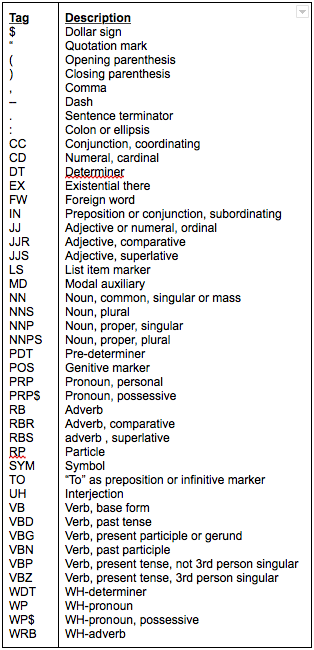
\includegraphics[width=\linewidth]{POStags}
   \captionof{figure}{Penn Treebank Tagset}
\end{Figure}   

Other systems were considered such as RASP (Robust Accurate Statistical Parsing) which is another system designed for syntactic annotation of free text. \cite{briscoe} It is implemented using C and Common Lisp and uses POS tags derived from the CLAWS tagset. The CLAWS tagset is comprised of over 130 tags depending on the version so it is much more extensive than the Penn Treebank Tagset. For example, the CLAWS tagset goes into finer detail with verbs specifying individual tags for the verbs to be, to do, and to have. It even goes so far as to break out each of these verbs to have a tag per verb tense. Because RASP uses a larger tagset, we deemed it to be beneficial to start with the simplest tagset available.

Another system we considered is the NLP software available from The Stanford NLP group. Like NLTK, it uses the Penn Treebank tagset but instead of being implemented in python, they use Java. In addition, the documentation available from NLTK is better which is why we chose NLTK over other systems.

% --------------------------------------------------------------------
\subsection{NLTK - Tagging Sentences}
% -------------------------------------------------------------------- 
In using NLTK, we are able to transform regular sentences into POS tags. There are four stages in this process from getting it from the initial sentence to a sentence with POS tags. Starting with initial sentences (1), it is necessary to convert this so each sentence is broken down to its individual sentences (2). This process is known as tokenizing sentences. The next step is to break each sentence into its individual words and punctuation which is called word tokenization (3). The final step is to tag each word in the sentence (4).

\begin{enumerate}
   \item Initial Sentence: `I went on a walk. It was nice outside.'
   \item Tokenize Sentence: [`I went on a walk.', `It was nice outside.']
   \item Tokenize Words: [[`I',`went',`on',`a',`walk',`.'], [`It',`was',`nice',`outside',`.']]
   \item Tag Words in Sentence: [(`I', `PRP'), (`went', `VBD'), (`on', `IN'), (`a', `DT'), (`walk', `NN'), (`.', `.')]
\end{enumerate}


% --------------------------------------------------------------------
\subsection{Project Gutenberg}
% --------------------------------------------------------------------
In order to build the rule set of correct tag sequences, literature from Project Gutenberg was used. \cite{gutenberg} Ten famous literature works were used. They were picked based on their popularity and the fact that the authors are all native English speakers. Because of their native English speaker and their world-wide renown, proper grammar is assumed. The ten pieces we used are as follows.

\begin{enumerate}
   \item \textit{The Adventures of Tom Sawyer} by Mark Twain
   \item \textit{Alice in Wonderland} by Lewis Carroll
   \item \textit{Emma} by Jane Austen
   \item \textit{Jane Eyre} by Charlotte Bronte
   \item \textit{Moby Dick} by Herman Melville
   \item \textit{The Picture of Dorian Gray} by Oscar Wilde
   \item \textit{Pride and Prejudice} by Jane Austen
   \item \textit{Sense and Sensibility} by Jane Austen
   \item \textit{A Tale of Two Cities} by Charles Dickens
   \item \textit{The Yellow Wallpaper} by Charlotte Perkins Gilman
\end{enumerate}

% --------------------------------------------------------------------
% --------------------------------------------------------------------
\section{Algorithm}
% --------------------------------------------------------------------
% --------------------------------------------------------------------


% --------------------------------------------------------------------
\subsection{Generating Rule Set}
% --------------------------------------------------------------------

\begin{enumerate}
   \item Import list of grammatically correct sentences
   \item Tokenize sentences
   \item Tag sentences - generate POS tags
   \item Extract POS tag sequences into txt file
  \end{enumerate}

% --------------------------------------------------------------------
\subsection{Grading Against Rule Set}
% --------------------------------------------------------------------
 To score an input sentence or sentences:
 
\begin{enumerate}
   \item Read sentence(s)/summary
   \item Tokenize sentence(s)
   \item Tag sentence(s) 
   \item Extract POS tag sequences
   \item Compare tag sequence generated from input sentence to existing rule set
   \item Score 1 = good grammar (found in rule set), Score 0 = bad grammar (not found)
  \end{enumerate}

% --------------------------------------------------------------------
% --------------------------------------------------------------------
\section{Results}
% --------------------------------------------------------------------
% --------------------------------------------------------------------
What results are we expecting?\\
0 for bad grammatical sentence\\
1 for good grammatical sentence\\

What have we seen?\\
Works for sentences/structures we know are in the text file.\\
Does not work on all grammatically correct sentences...yet\\



% --------------------------------------------------------------------
% --------------------------------------------------------------------
\section{Limitations}
% --------------------------------------------------------------------
% --------------------------------------------------------------------
When creating the text file of correct POS tag sequences, it became apparent that it would continue to grow significantly no matter how many sentences were already included in the file. When added the ten books to it, it was apparent that there is not much overlap in sentence structure between each book. For example, the total number of sentences in all ten books is 58,895 while the tag sequences file has 56,025 sentences. This is a difference of only 2,870 meaning that between ten novels, there is only an overlap of about 5\%. This result is a clear example of the infiniteness of language. When discussing sentence construction in the NLTK documentation \cite{nltk}, they comment on how easy it is to ``extend sentences indefinitely." They go on to say ``it's not hard to concoct an entirely novel sentence, one that has probably never been used before in the history of the language." Because of the infiniteness of language, grammatically correct sentences that are not in the list of grammatically correct sequences is entirely possible.



Infiniteness of language\\
Text file becoming too big\\
Limitations on books used\\

% --------------------------------------------------------------------
% --------------------------------------------------------------------
\section{Conclusion}
% --------------------------------------------------------------------
% --------------------------------------------------------------------
Conclusion

% --------------------------------------------------------------------
% --------------------------------------------------------------------
\section{Future Work}
% --------------------------------------------------------------------
% --------------------------------------------------------------------
Future work

\newpage

\bibliography{references}
\bibliographystyle{ieeetr}

\end{multicols}
\end{document}
